\documentclass{article}
\usepackage[margin=1in]{geometry}
\usepackage{amsmath, amssymb, amsthm}
\usepackage{enumitem}

% colored links
\usepackage{hyperref}
\hypersetup{
    colorlinks=true,
    linkcolor=blue,
    filecolor=magenta,      
    urlcolor=blue,
    }



% Inputting Python code
\usepackage[dvipsnames]{xcolor}
\definecolor{textblue}{rgb}{.2,.2,.7}
\definecolor{textred}{rgb}{0.54,0,0}
\definecolor{textgreen}{rgb}{0,0.43,0}
\usepackage{upquote}
\usepackage{listings}
\lstset{
    language=Python, 
    tabsize=4,
    basicstyle={\ttfamily},
    keywordstyle=\color{textblue},
    commentstyle=\color{textgreen},
    stringstyle=\color{textred},
    frame=none,
    columns=fullflexible,
    keepspaces=true,
    showstringspaces=false,
    xleftmargin=-15mm, % manual adjustment, figure out permanent solution
}

%Creating algorithms
\usepackage{algorithm}
\usepackage[noend]{algpseudocode}

\usepackage{tcolorbox}
\tcbuselibrary{skins,hooks}
\usetikzlibrary{shadows}
\usepackage{lipsum}

%Images
\usepackage{graphicx}
    \usepackage{subcaption}
    \usepackage{float}
    % \usepackage[labelsep=period]{caption}

    
%Creating Figures
\usepackage{tikz}
\usetikzlibrary{calc, math, matrix, graphs, positioning}


% the settings of tikz is used for the optimization of the graphs  
\usetikzlibrary{shapes, arrows, calc, arrows.meta, fit, positioning} % these are the parameters passed to the library to create the node graphs  
\tikzset{  
    -Latex,auto,node distance =1.5 cm and 1.3 cm, thick,% node distance is the distance between one node to other, where 1.5cm is the length of the edge between the nodes  
    state/.style ={ellipse, draw, minimum width = 0.9 cm}, % the minimum width is the width of the ellipse, which is the size of the shape of vertex in the node graph  
    point/.style = {circle, draw, inner sep=0.18cm, fill, node contents={}},  
    bidirected/.style={Latex-Latex,dashed}, % it is the edge having two directions  
    el/.style = {inner sep=2.5pt, align=right, sloped}  
}  

%Formatting and Spacing
\setitemize[1]{noitemsep, parsep = 5pt, topsep = 5pt}
\setenumerate[1]{label = (\alph*), parsep = 1pt, topsep = 5pt}
\setlength\parindent{0pt}
\linespread{1.1}

% title
\title{\vspace{-1cm}CS 2051: Honors Discrete Mathematics \\Spring 2023 Homework 5 Supplement}
\author{Sarthak Mohanty }
\date{}

\begin{document}

\maketitle

\section*{Overview}

   \qquad Traditionally, computer software has been written for serial computation: instructions corresponding to a tasks are executed on one processing unit at a time. However, nowadays many computational tasks consist of many elementary operations, some of which have to be computed sequentially, while others can be computed in parallel.

    \vspace{2mm}
    \qquad In a distributed or high performance computing course, one of the first things you may learn is \href{https://en.wikipedia.org/wiki/Amdahls_law}{Amdahl’s law}, which gives a quantitative measure of the speedup $S$ -- i.e., how much faster the task can be performed by using $n$ parallel processors: $$S = \frac{1}{1 - p + \frac{p}{n}}.$$ Here, $p$ is the proportion of operations that can be performed in parallel.


    \vspace{2mm}
    \qquad However, it is not typically the case that we can classify operations simply as “parallel” or “sequential.” Instead, a task might consist of several sub-tasks, some of which need to be completed before others are started. Optimally scheduling these tasks is much trickier, and is currently an area of \href{https://www.cs.umd.edu/~samir/DCscheduling18/slides/Janardhan Kulkarni.pdf}{active research}. However, with the right mathematical foundations, we can at least start to understand the complexity of task scheduling, and begin to develop efficient strategies for tackling ``easy" versions of the problem.

    \vspace{2mm}
    \qquad In this supplement, you learn about a generalized form of functions known as \textbf{relations}, and explore the connection between functions and relations. You'll then learn about two important types of relations, including \textbf{equivalence relations} and \textbf{partial orders}. Finally, we'll explore some of the applications of these concepts, including a return to our original problem of multi-processor scheduling.

\section*{Part 1: Generalizing Functions with Relations}

    This week, you learned about functions. We (informally) defined them as a well-defined mapping between two sets. However, what about mappings that are not well-defined? Is there no way to represent these? As a matter of fact, there is!
    
    \vspace{3mm}
    \textbf{Definition.} a \textit{relation} $\mathcal{R}$ over sets $A, B$ is a subset of $A \times B$. The notation $a\mathcal{R}b$ or $a \sim b$ is often used to denote that $(a, b) \in \mathcal{R}$.

    \subsection*{Easy Examples}
    
    Let $\mathcal{R}_1, \dots, \mathcal{R}_4$ be a relation on $A = \{1, 2, 3, 4\}$.
    \begin{itemize}
        \item $\mathcal{R}_1 = \{(a, b) \mid a \le b)\}$
        \item $\mathcal{R}_2 = \{(a, b) \mid a = b)\}$
        \item $\mathcal{R}_3 = \{(a, b) \mid a+b \le 2022)\}$
        \item $\mathcal{R}_4 = \{(a, b) \mid a \text{ divides } b\}$
    \end{itemize}

    \subsection*{Another Example: Functions}
    Functions are also an example of relations. Specifically, a function is any relation $\mathcal{R}: A \rightarrow B$ with the property that for any $x$ there is exactly one $y$ such that $x\mathcal{R}y$.
    
    
\subsection*{Properties of A Relation $\mathcal{R} \colon A \rightarrow A$}

    \begin{enumerate}[align=left]
        \item [\textbf{Reflexitivty}] $\mathcal{R}$ is \textit{reflexive} if 

        $(\forall a \in A)(a\mathcal{R}a)$

        ``Everyone has slept with themselves"
        \item [\textbf{Symmetry}] $\mathcal{R}$ is \textit{symmetric} if 

        $(\forall a, b \in A)(a\mathcal{R}b \iff b\mathcal{R}a)$

        ``If $a$ slept with $b$, then $b$ slept with $a$"

        \item [\textbf{Antisymmetry}] $\mathcal{R}$ is \textit{symmetric} if 

        $(\forall a, b\in A)(a\mathcal{R}b \wedge b\mathcal{R}a \rightarrow a=b)$

        ``No pair of distinct people have slept with each other"

        \item [\textbf{Transitivity}] $\mathcal{R}$ is \textit{transitive} if 

        $(\forall a, b, c\in A)(a\mathcal{R}b \wedge b\mathcal{R}c \rightarrow a\mathcal{R}c)$

        ``If $a$ slept with $b$ and $b$ slept with $c$, then $a$ slept with $c$ too."
    \end{enumerate}

    When a relation is reflexive, antisymmetric, and transitive, we call it a \textit{partial order}. When a relation is reflexive, symmetric, and transitive, we call it a \textit{equivalence relation}.

    \vspace{3mm}
    \begin{tcolorbox}[colback=yellow!30]
        In this part, you'll implement the functions \lstinline{isPartialOrder(elements, relation)} and \lstinline{isEquivalenceRelation(elements, relation)}. These functions takes in a relation (represented as a set of tuples) and returns whether or not the relation (taken over the set of elements) is a valid partial order or equivalence relation, respectively. You must use the following helper methods:
        \begin{itemize}
            \item \lstinline{isReflexive(elements, relation)}
            \item \lstinline{isSymmetric(elements, relation)}
            \item \lstinline{isAntisymmetric(elements, relation)}
            \item \lstinline{isTransitive(elements, relation)}
        \end{itemize}
        \textbf{All methods (and all helper methods) must be implemented in one line.}
        
        Tip: Use the \lstinline{all()} method
    \end{tcolorbox}



\section*{Part 2: Partitioning with Equivalence Relations}
    In the world of computer science, there are two main applications for relations: partitioning and scheduling. In this part, we'll cover partitioning, which is essentially just a reframing of our knowledge about equivalence relations.

    \vspace{2mm}
    \textbf{Definition}: Given some relation $\mathcal{R}$ over the set $A$, the \textit{equivalence class} of an element $x \in A$ is $$[x] = \{y : x \mathcal{R} y\}$$

    These equivalencies have a very important theorem

    \begin{tcolorbox}
        \textbf{Theorem}: The equivalence classes of an equivalence relation on a set $A$ \textit{partition} $A$ into a collection of disjoint, nonempty subsets $A_{1}, A_{2}, \dots, A_{n}$ such that (and this is the important part) $\bigcup _{i = 1}^{n} = A$.
    \end{tcolorbox}
    
    \vspace{2mm}
    Ok, so this fact is cool and all, but what's the point? Well, if we have say a million elements in a set, but only three equivalence classes, we need only consider the three classes to understand the properties of the entire set. This is where the concept of \textit{canonical forms} comes in, which refers to the standard representation of a set in terms of its equivalence classes, making it easier to analyze and manipulate. The following examples provide more context onto these definitions.

    \subsection*{Example: Congruence Relations}
        Our first example delves into \textit{number theory}, a field you will become more intimate with in the next few supplements. Informally, define the relation $a\mathcal{R}_{n}b$ over $\mathbb{Z} \times \mathbb{Z}$ if $a$ and $b$ have the same remainder when divided by some number $n$. We usually denote this using $$a \equiv b \pmod{n}.$$ For example, $-10$ and $15$ are related under $\mathcal{R}_{5}$, $$-10 \equiv 15 \pmod{5},$$ since $-10 - 15 = -25$ is a multiple of $5$, or equivalently since both $-10$ and $15$ have the same remainder $0$ when divided by $5$.
        
        \vspace{2mm}
        All such relations $\mathcal{R}_{n}$ are equivalence relations, and partition the set of integers into $n$ equivalence classes. For example, the relation $\mathcal{R}_{3}$ partitions the integers like so
        \begin{gather*}
            \{\dots, -7, -4, -1, 2, 5, 8, \dots\} \\
            \{\dots, -8, -5, -2, 1, 4, 7, \dots\} \\
            \{\dots, -6, -3, 0, 3, 6, 9, \dots\}
        \end{gather*}
        The canonical forms for each of these sets are $2$, $1$, and $3$ respectively (try to spot why!)


    \subsection*{Example: Vector Spaces}
        One of the most prominent uses of equivalence classes is in linear algebra. After all, it's very difficult to determine when two vector spaces or matrices are functionally ``identical". 

        \vspace{3mm}
        If you've taken an introductory linear algebra course, you learned about Gauss's Method to solve a system of equations. In essence, it worked by starting with a matrix and deriving a sequence of other matrices, each \textit{row equivalent} to each other. It turns out that row equivalence is an equivalence relation, and partitions the set of all matrices into corresponding classes, as shown in Figure (\ref{fig:2}).

        \vspace{3mm}
        We can generalize this one step further with a relation known as \textit{matrix equivalence}. Matrix equivalent matrices represent the same map, with respect to appropriate pairs of bases. Matrix equivalence classes are also characterized by rank: two same-sized matrices are matrix equivalent if and only if they have the same rank. In fact, matrix similarity is a special case of matrix equivalence!

        \vspace{3mm}
         The canonical forms for row equivalence are the Reduced Echelon form matrices, which you may already be familiar with. Meanwhile, the canonical forms for matrix similarity are Jordan Normal forms. (the canonical forms for matrix equivalence are a bit more complicated.)
        
        \begin{figure}[H]
            \centering
            \begin{subfigure}{0.45\textwidth}
                \centering
                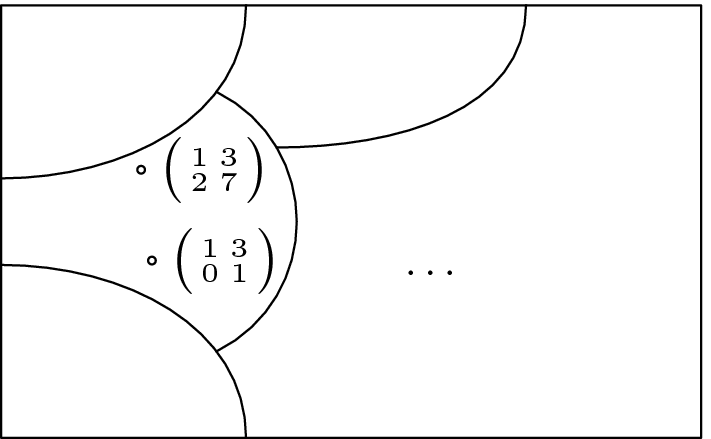
\includegraphics[scale = .22]{sp23/hw-supplements/hw5-supp/images/linalg_reduced_echelon_form_equiv_classes.png}
                \caption{Two matrices with the same row space.}
            \end{subfigure}
            \begin{subfigure}{0.45\textwidth}
                \centering
                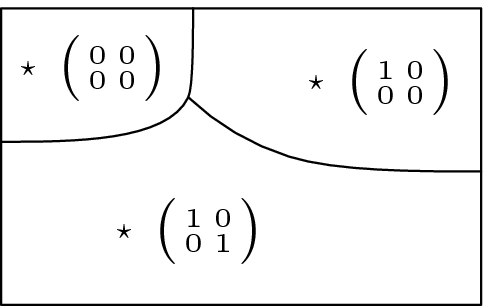
\includegraphics[scale = .33]{sp23/hw-supplements/hw5-supp/images/linalg_2by2_rank_equivalence_classes.png}
                \caption{The canonical forms for the set of $2 \times 2$ matrices.}
            \end{subfigure}
            \caption{Row equivalence as an equivalence relation.}
            \label{fig:2}
        \end{figure}

        \begin{figure}[H]
            \centering
            \begin{subfigure}{0.45\textwidth}
                \centering
                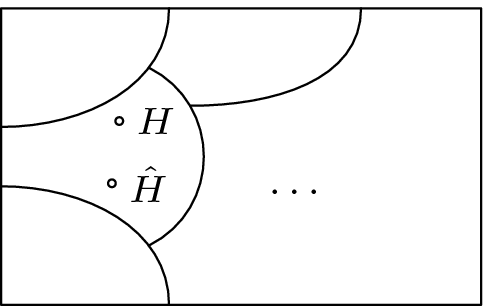
\includegraphics[scale = .3]{sp23/hw-supplements/hw5-supp/images/linalg_matrix_equivalence_classes.png}
            \end{subfigure}
            \begin{subfigure}{0.45\textwidth}
                \centering
                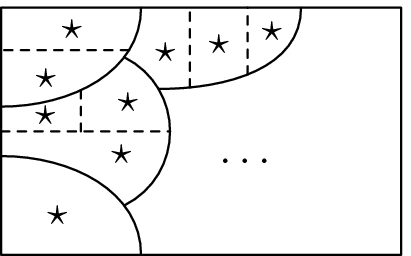
\includegraphics[scale = .36]{sp23/hw-supplements/hw5-supp/images/linalg_matrix_similarity_equiv_classes.png}
            \end{subfigure}
            \caption{Matrix similarity is a finer partition than matrix equivalence}
            \label{fig:1}
        \end{figure}

    \vspace{3mm}
    \begin{tcolorbox}[colback=yellow!30]
        \textbf{In this part, you'll implement the following function:}
        \begin{itemize}
            \item \lstinline{partition(elements, relation)}: This function takes a equivalence relation (this time represented as a boolean function), and returns a partition of the elements into equivalence classes. For example, given the congruence relation described above, the function should return
        \begin{lstlisting}[belowskip=-10pt]
            >>> partition([i for i in range(-8, 8)], lambda x, y: (x - y) % 3 == 0)
            [{-6, -3, 0, 3, 6}, {-8, -5, -2, 1, 4, 7}, {-7, -4, -1, 2, 5, 8}]
        \end{lstlisting}

        \end{itemize}

        Tip: iterating over sets is difficult. Try casting.
    \end{tcolorbox}

    % idea: quotient graph https://networkx.org/documentation/stable/_modules/networkx/algorithms/minors/contraction.html#equivalence_classes

\section*{Part 3: Single-Processor Task Scheduling}

    We now delve into partial orderings, or ``posets". We'll cover a nice \textit{graph}ical representation of posets, and then cover their applications in the context of task scheduling. 
    

    \subsection*{Dependency Graphs}
    
    To start, let's consider the following story. 

    \begin{tcolorbox}[colback=red!20]
        You're a recently admitted CS major at Georgia Tech. To save money, you're trying to graduate as early as possible.  You have a lot of course that you can take, but you're not sure which ones to take when. Furthermore, many of the courses are dependent upon completion of other courses (for example, CS 1332 requires CS 1331, which in turn requires CS 1301). How long will it take for you to graduate?
    \end{tcolorbox}

    We can represent this problem as a poset $\mathcal{R}$ over the set of courses $A$, where $a \mathcal{R} b$ iff $a$ is a prerequisite to take $b$:

    \begin{center}
    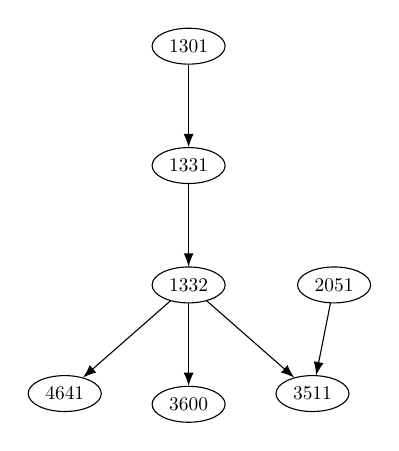
\begin{tikzpicture}[scale = 0.7, transform shape]  
        % a is the name of the node and A is the text inside the node/vertex  
        \node[state] (1301) at (0,0) {1301}; % here, state signifies that the shape of the node will be the shape declared in the above state/.style command.  
      
        % you can mention any location such as right, left, above, below, etc.  
         
        \node[state] (1331) [below =of 1301] {1331};  
        \node[state] (1332) [below =of 1331] {1332};
        \node[state] (2051) [right =of 1332] {2051};  
        \node[state] (4641) [below left =of 1332] {4641};  
        \node[state] (3600) [below =of 1332] {3600};  
        \node[state] (3511) [below right =of 1332] {3511};  
        \path (1301) edge (1331); % it is the path of the edge from one node to another  
        \path (1331) edge (1332);
        \path (1332) edge (4641);
        \path (1332) edge (3600);
        \path (1332) edge (3511);
        \path (2051) edge (3511);
      
        % % Bidirected edge  
        % \path[bidirected] (1331) edge[bend left=60] (1332); % this is the basic command in this code. It is used to draw the curved edge with a certain angle. You can change the angle according to the requirements.  
          
        % \path (a) edge (c);  
        %  \path[bidirected] (a) edge[bend right=60] (c);  
        %  \draw (b) -- (c);  
          
    \end{tikzpicture}  
    \end{center}
    This is known as a \textit{dependency graph}.



    % We can model these dependencies as a partial ordering. For example, the partial ordering (do one on classes) can be represented as a dependency graph, which in turn can be represented as a dependency list. (show illustration). Note how we


    \subsection*{Task Scheduling}
    
    Using the formalism of posets, we can also define the problem of computing an optimal schedule.

    \vspace{3mm} Assume that some task $T$ can be decomposed into sub-tasks $T = \{T_{1}, T_{2}, \dots, T_{n}\}$. In general, we can encode the relationships between the various $T_{i}$ as a poset, where $T_{i} \prec T_{j}$ if (sub)task $T_{i}$ needs to be performed before $T_{j}$. \textbf{Assume each task $T_{i}$ takes 1 unit of time to complete.} Given $k$ processors $P_{1}$, $P_{2}$, \dots, $P_{k}$ a \textbf{schedule} for $T$ assigns each sub-task $T_{i}$ a processor $P_{j}$ as well as a time $t_{i}$ at which $P_{j}$ should start task $T_{i}$. Observe that if a processor starts $T_{i}$ at times $t_{i}$, then the task will complete at time $t_{i} + 1$. A schedule is \textbf{feasible} if:
    \begin{enumerate}[label = \arabic*]
        \item no single processor is performing multiple tasks at the same time (i.e., if a processor is assigned $T_{i}$ and $T_{j}$ at times $i, j$, then $i \ne j$) and
        \item for every pair of tasks $T_{i}$ and $T_{j}$ with $T_{i} \prec T_{j}$, task $T_{j}$ is scheduled to start some time after (or at the same time) $T_{i}$ completes. (i.e.\ $T_{i} \prec T_{j} \Rightarrow t_{j} > t_{i}$)
    \end{enumerate}

    \subsection*{Topological Sorting}
    If we have only one processor, then the answer is fairly simple, just create a topological sorting. 
    
    \underline{The proof for this statement will be added in a future update.}
    
    \vspace{3mm}
    \textbf{Definition}: A topological sorting is a total ordering of a partially ordered set.

    \vspace{3mm}
    We present a common algorithm for finding the topological sort below, known as Kahn's algorithm. (Note: the pseudocode refers to \textit{minimal elements}. These are simply all elements $v$ such that there is no other element $u$ such that $(u, v) \in \mathcal{R}$)

    

    \begin{algorithm}
        \caption{\textsc{KahnsAlgorithm}$(elements, poset)$}\label{alg:cap}
        \label{alg:topological_sort}
        \begin{algorithmic}
            \State $T = \emptyset$
            \State $S = $ all minimal elements in $poset$
            \While{$S \ne \emptyset$}
                \State $u = $ an element in $S$
                \State $S = S - \{u\}$
                \State $T = T \cup \{u\}$
                \State $uv\_dependencies = \{(u, v) : v \in elements \text{ and }(u, v) \in poset\}$
                \For{each $(u, v)$ in $uv\_dependencies$}
                    \If {v is minimal} insert $v$ in $S$ \EndIf
                \EndFor

            \EndWhile
            
                
            \State \Return{T}
        \end{algorithmic}
    \end{algorithm}


    \vspace{3mm}
    \begin{tcolorbox}[colback=yellow!30]
        \textbf{In this part, you'll implement the following function:}
        
        \lstinline{topological_sort(poset)}: This method takes in a partially ordered set defined on \lstinline{elements} (in the form of a dependency list) and returns a valid topological sort. We can use it to solve our course scheduling dilemma above:

        \begin{lstlisting}[belowskip=-10pt]
            >>> topological_sort({'1301', '1331', '1332', '4641', '2051', '3600', '3511'},
                    {('1301', '1331'), ('1331', '1332'), ('1332', '4641'),\
                     ('2051', '3511'), ('1332', '3511'), ('1332', '3600')})
                ['2051', '1301', '1331', '1332', '4641', '3511', '3600']
        \end{lstlisting}
    \end{tcolorbox}

\section*{Part 4: Multi-Processor Task Scheduling}

    \textbf{Definition} A \textit{chain} is such that every distinct pair of elements is comparable in $\mathcal{P}$.

    Note that the time it takes to schedule tasks, even with an unlimited number of processors, is at least the length of the longest chain. Indeed, if we used less time, then two items from a longest chain would have to be done at the same time, which contradicts the precedence constraints. 


    \vspace{2mm}
    The nice thing about posets is that this is always possible! In other words, for any poset, there is a legal paralle schedule that runs in $t$ steps, where $t$ is the length of the longest chain. This is known as Mirsky's theorem:
    
    \underline{The proof for this statement will be added in a future update.}

    \vspace{2mm}    
    The case where there are a limited number of processors, however, is more useful in practice, as we'll see below.

    \begin{tcolorbox}[colback=yellow!30]
        \textbf{In this part, you'll implement the following function:}
        \begin{itemize}
            \item \lstinline{generate_schedule(elements, poset, num_processors)}:  This method will solve the original problem defined in ``Task Scheduling". It should return a valid schedule in the form of a list of lists, where the $i$-th element in the list represents the jobs we should schedule at time $t = i$.

        If, for instance, we could take two courses a semester, we could generate an optimal schedule as follows:
    \begin{lstlisting}[belowskip=-10pt]
        >>> generate_schedule({'1301', '1331', '1332', '4641', '2051', '3600', '3511'},
                {('1301', '1331'), ('1331', '1332'), ('1332', '4641'),\
                 ('2051', '3511'), ('1332', '3511'), ('1332', '3600')}, 2)
            ['1301', '2051'], ['1331'], ['1332'], ['4641', '3600'], ['3511']]]
    \end{lstlisting}
        \end{itemize}
        Tip: If you've implemented the previous part correctly, this part should just be a few modifications.
        
    \end{tcolorbox}



    \section*{(Optional) Part 5: Processor Optimization}
    What if we wanted to optimize the number of processors? In other words, what is the minimum number of processors such that increasing the number of processors does not decrease our latency? In the course scheduling example, it was easy to see that the optimal number of processors was $3$ by just looking at the dependency graph above. 
    
    
    \subsection*{Brute Force}
    If we wanted to do this in general, one way would be to run \lstinline{generate_schedule} for all \lstinline{num_processors} from $1$ to \lstinline{len(elements)}, and then return the minimum.


    \subsection*{Improvements and Further Reading}
    \vspace{3mm}
    However, note that this algorithm is not efficient, since there is the possibility that we have to run \lstinline{generate_schedule} many times. It seems natural to assume there is an efficient solution to this problem, and in fact there is! However, the details of the algorithm are far outside the scope of the course. If you really want to know, the details can be found in the \href{https://www.appliedcombinatorics.org/book/s_flowapplications_chain-partition.html}{MATH 3012 textbook}.
    
    % \textbf{(warning: even most 3012 professors don't get far enough to cover this topic, so this is really advanced stuff!)}
    
    \vspace{3mm} This processor optimization problem is also known as the \textit{dual} problem of Part 3. Duality is a fundamental concept in computer science, and you'll encounter it again in your Algorithms courses.


%     \subsubsection*{Incorrect Approach for processor optimization}

%     using the previous section, i'm sure many of you are picturing the following approach
    
%     apply a topological sort on the DAG
%     traverse over the nodes by the topological order, calculate the minimum level:
%     no parents: 0
%     otherwise: minimum parent level + 1
%     return the max level width (max num of nodes assigned the same level).

%     However, this approach does not always work. For a salient counterexample, consider a tree.

%     also discuss how bfs wouldnt work\

\section*{Submission Instructions (10 pts)}
    After you fill the appropriate functions, submit the following files to Gradescope and make sure you pass all test cases:
    \begin{itemize}
        \item \lstinline{relations.py}
        \item \lstinline{scheduler.py}
    \end{itemize}

    \vspace{3mm}
    \textbf{Notes}

    \begin{itemize}
        \item The autograder may not reflect your final grade on the assignment. We reserve the right to run additional tests during grading.
        \item Do not import additional packages, as your submission may not pass the test cases or manual review.
    \end{itemize}
    

\end{document}